\section{Exercise 2 - Design Patterns}
\subsection{Exercise 2.1 - Strategy Pattern}
Before this sprint iteration, the project already contained a small implementation of the strategy pattern. The MovableUnit interface was already there to provide methods a Unit should implement if it can move on the screen.\\

Since not every Unit can move, it is more flexible to add an interface for this. 
The methods for moving are not needed in classes such as Barricade. 
Instead of adding these methods in the superclass, it is better to add them in an interface so only subclasses implementing the interface, implement the methods.\\

The same can be done for shooting, and activating a unit on the player (such as a powerup).
The project was extended to include an interface for shooting, ShootingUnit and an interface for activating a unit on the player, ActivatableUnit. 

\subsection{Exercise 2.2 - Strategy Pattern}

\begin{figure}[ht!]
\centering
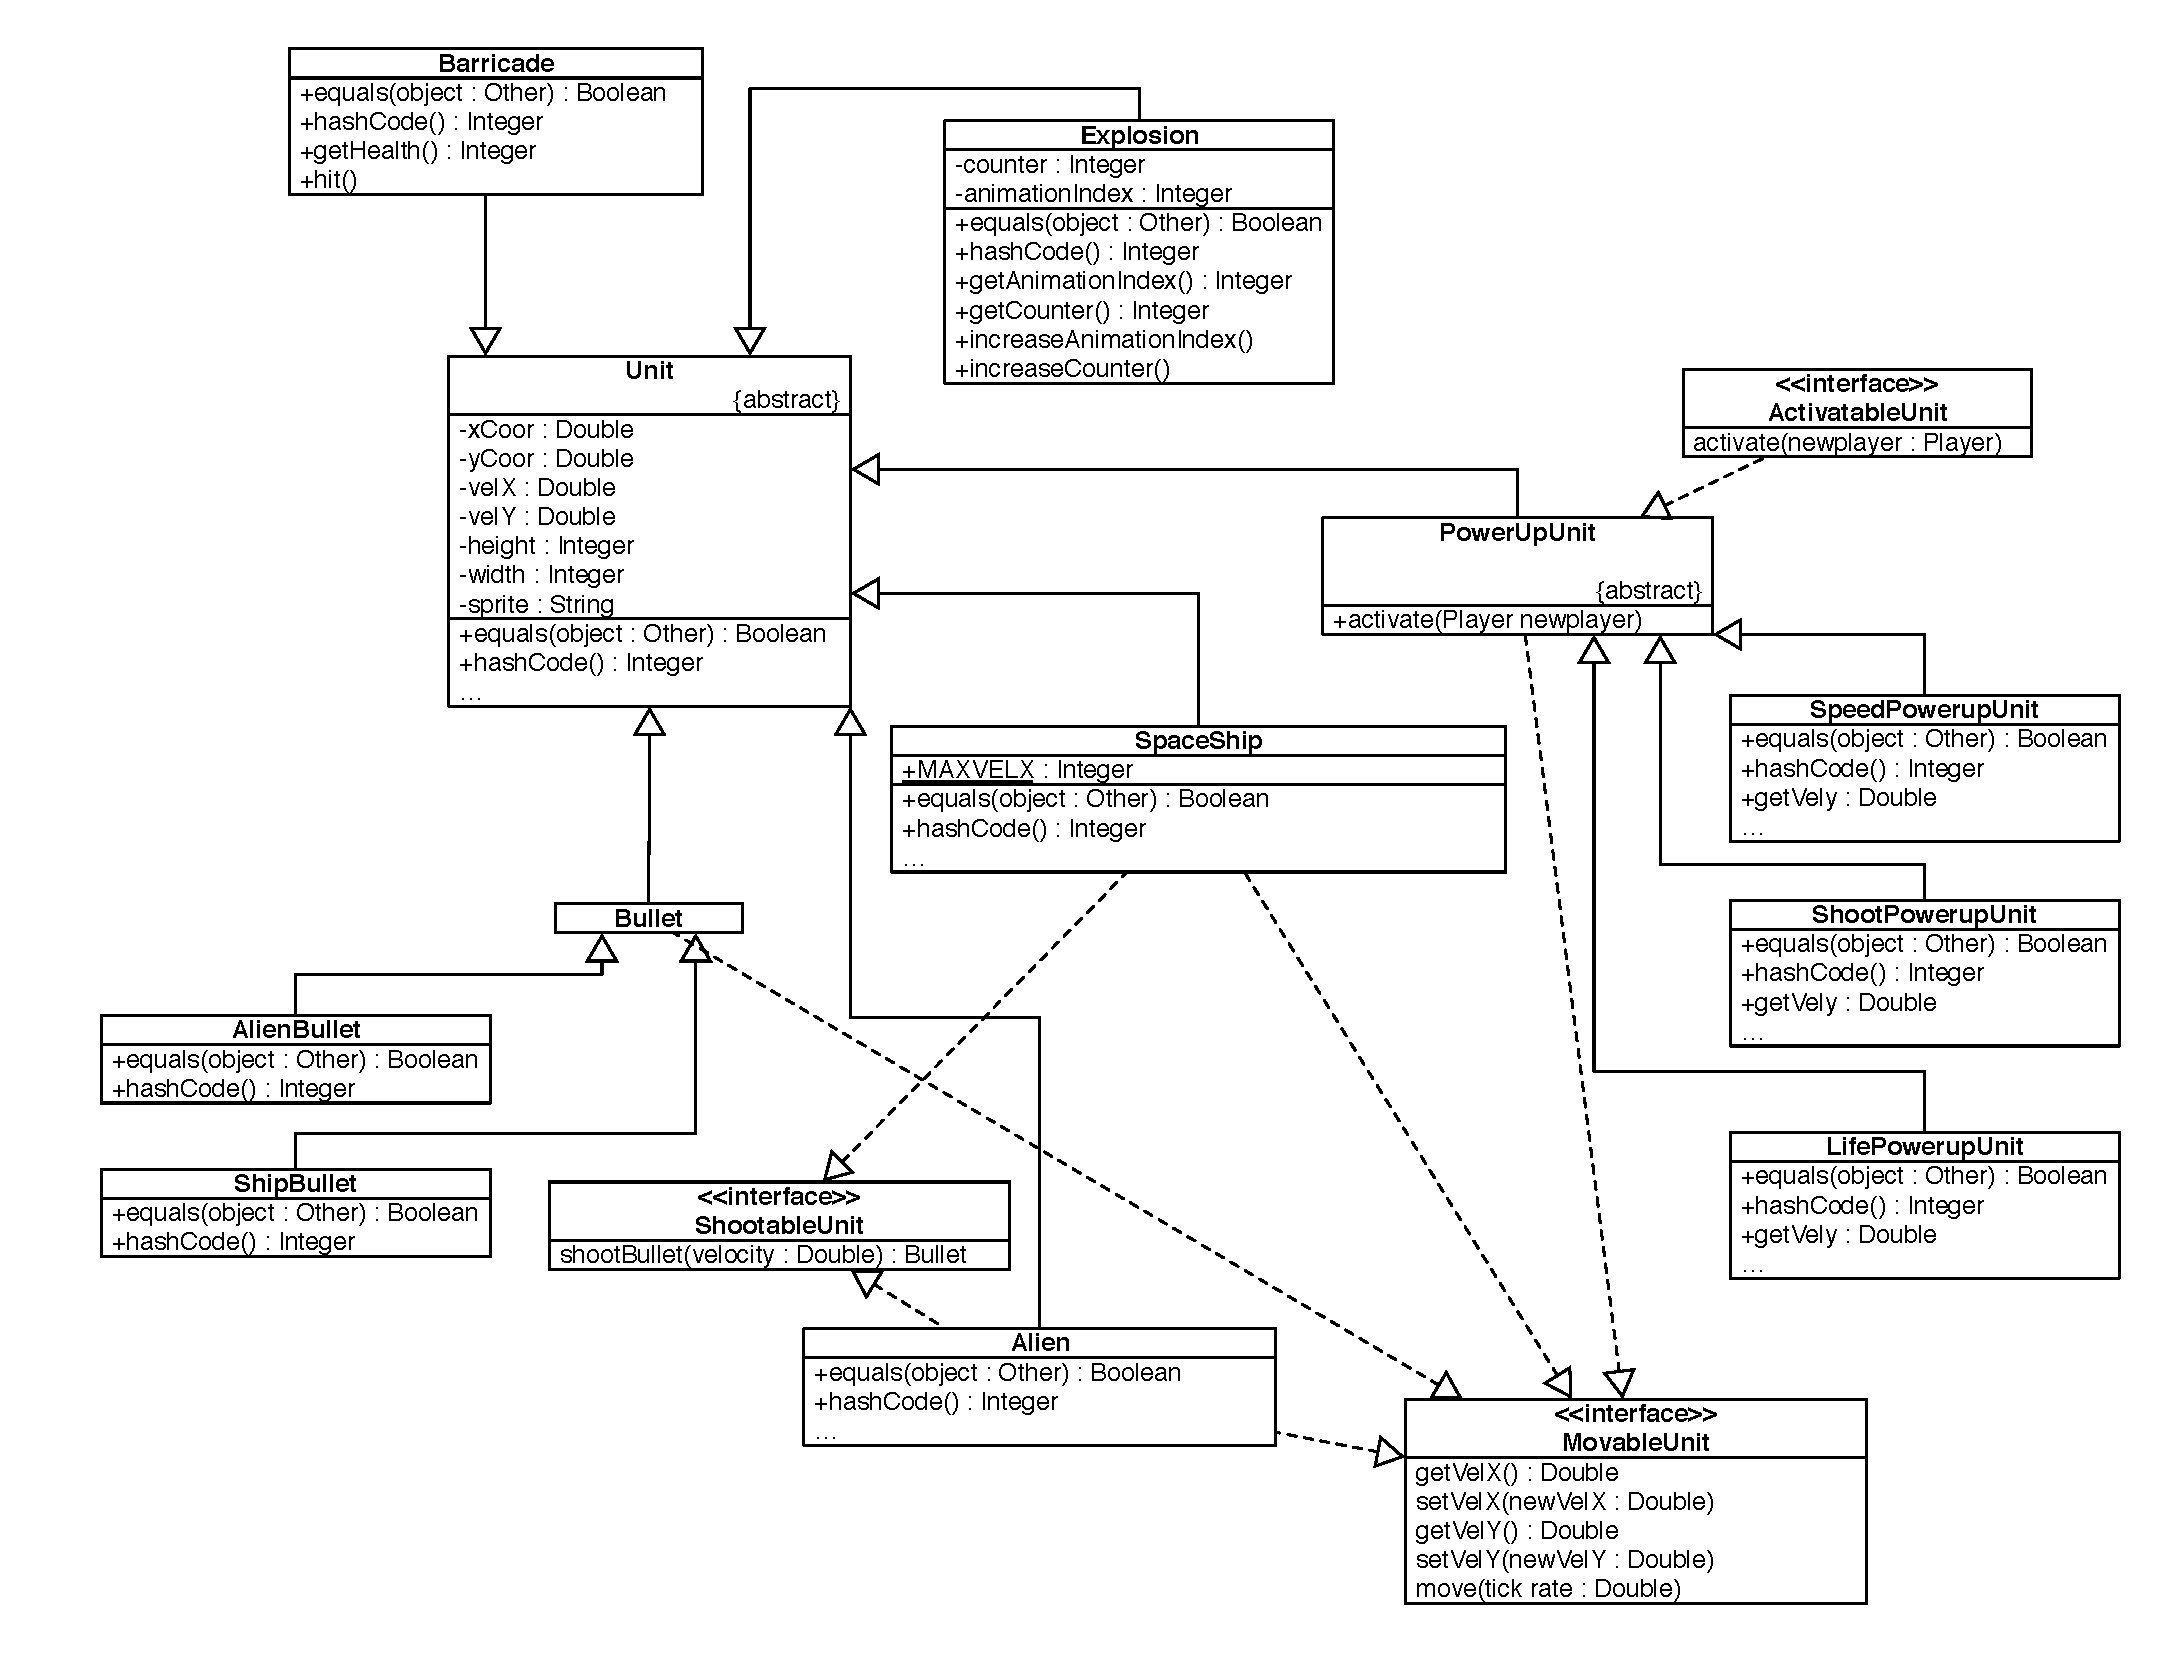
\includegraphics[width=15cm]{SI-UMLunitStrategy.pdf}
\caption{Strategy Pattern UML Class Diagram}
\label{fig:2-2strategy}
\end{figure}

Figure \ref{fig:2-2strategy} contains the UML Class diagram for the strategy pattern in Unit.

\subsection{Exercise 2.3 - Strategy Pattern}

\begin{figure}[ht!]
\centering
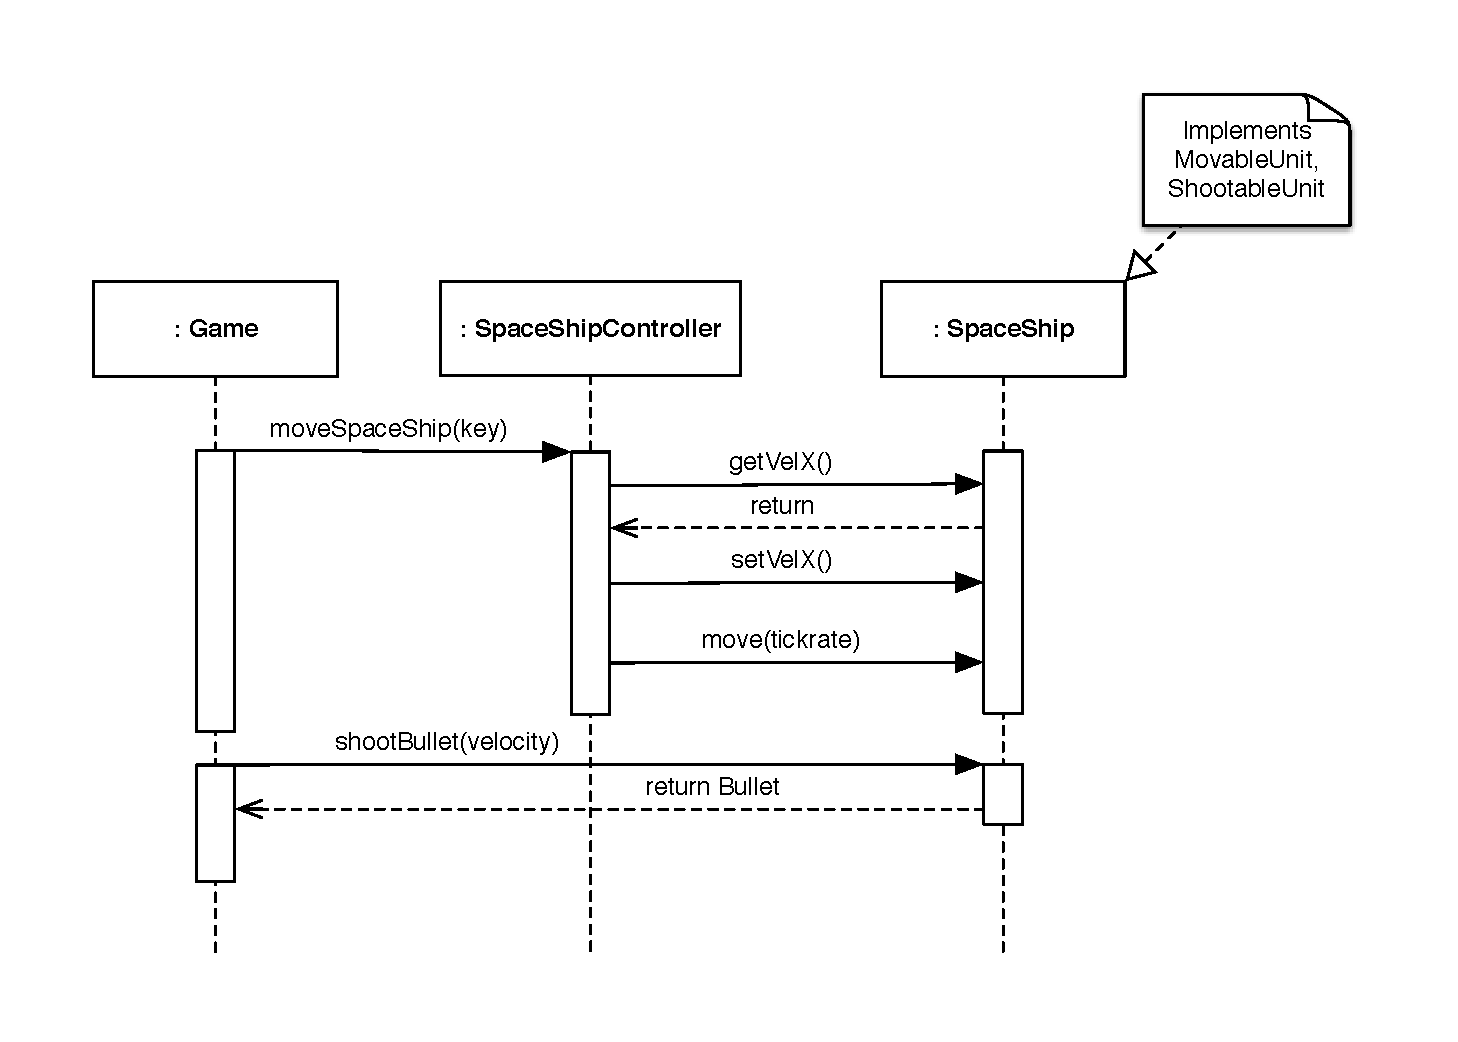
\includegraphics[width=15cm]{SI-Sequence-Strategy.pdf}
\caption{Strategy Pattern UML Sequence Diagram}
\label{fig:2-3strategy}
\end{figure}

Figure \ref{fig:2-3strategy} contains the UML Sequence diagram for the strategy pattern in Unit. This diagram only contains the case concerning MovableUnit and ShootingUnit. It visualizes that all methods defined in the interfaces are implemented and used correctly.

\subsection{Exercise 2.1 - Abstract Factory Pattern}
A factory pattern can be useful for the creation of a PowerUpUnit. If a powerup is created in game, it does not need knowledge of the implementation. In the project, there are three 'flavors' of powerups, Speed, Life and Shoot. If a factory is used, the factory handles the creation of each powerup and the game can easily obtain it by calling a method on the corresponding factory.\\

In the project, an interface AbstractPowerupFactory was created. The interface defines a create method which should be implemented. Three factories: LifePowerupFactory, SpeedPowerupFactory and ShootPowerupFactory implement this interface and create the corresponding powerups. In the PowerUpController, these three factories are used for the creation of the required powerup, instead of calling the constructor. 

\subsection{Exercise 2.2 - Abstract Factory Pattern}

\begin{figure}[ht!]
\centering
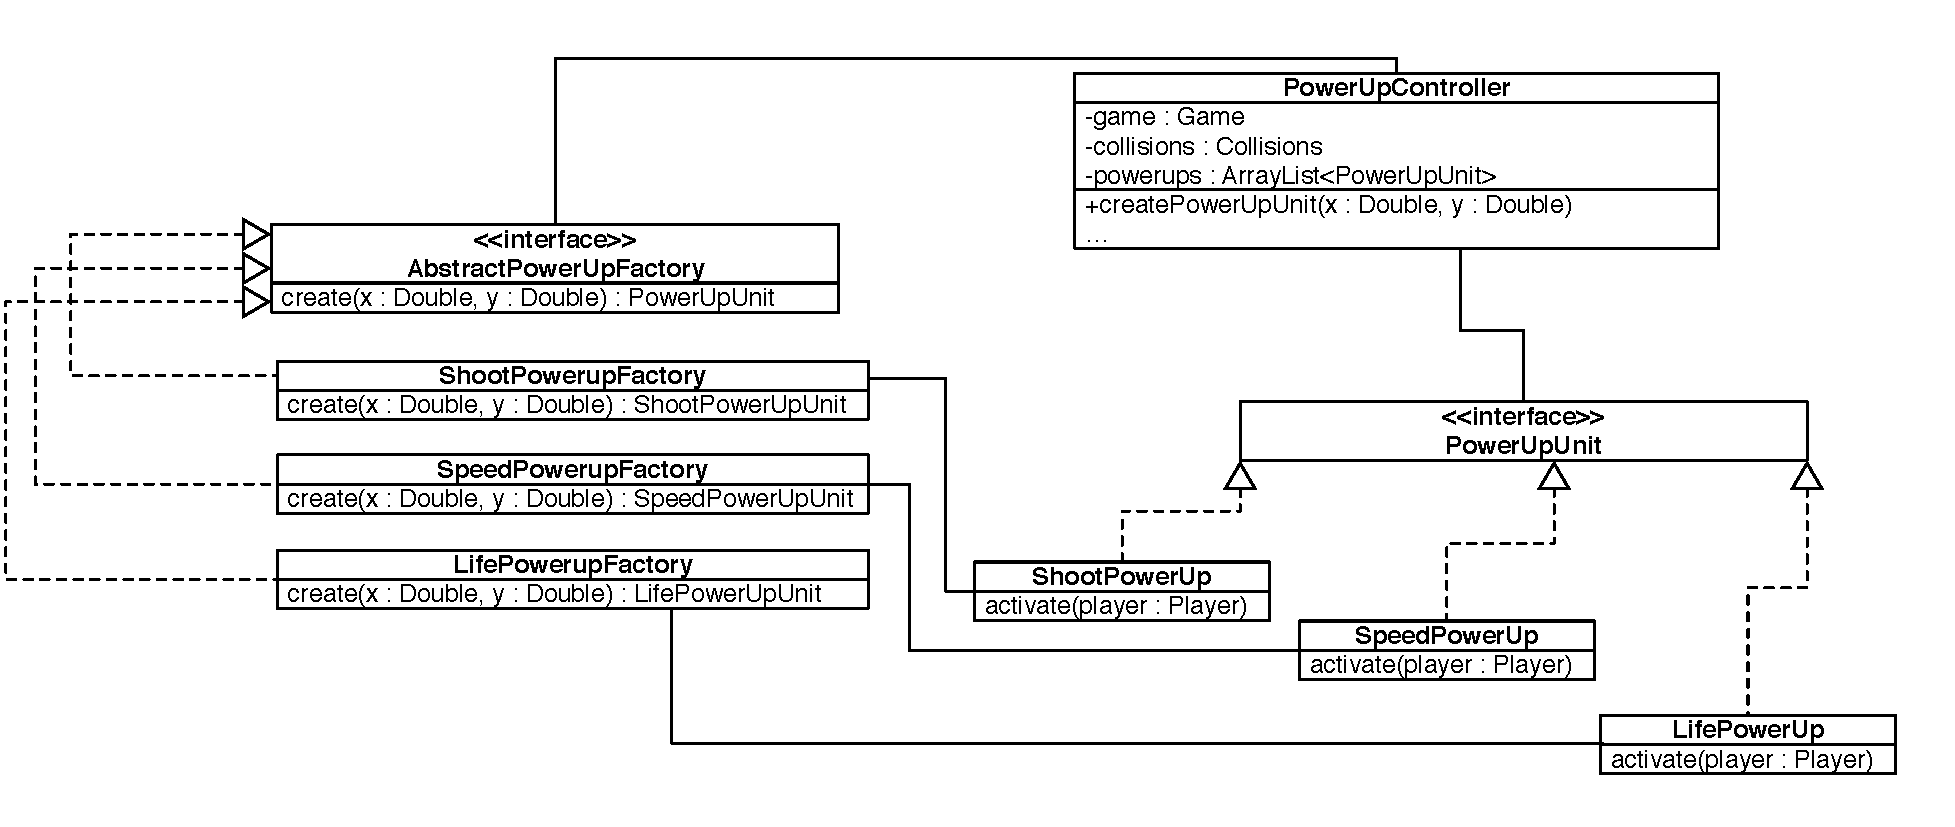
\includegraphics[width=15cm]{SI-UMLpowerupFactory.pdf}
\caption{Abstract Factory Pattern UML Class Diagram}
\label{fig:2-2factory}
\end{figure}

Figure \ref{fig:2-2factory} contains the UML Class diagram for the abstract factory pattern concerning the powerups.

\subsection{Exercise 2.3 - Abstract Factory Pattern}

\begin{figure}[ht!]
\centering
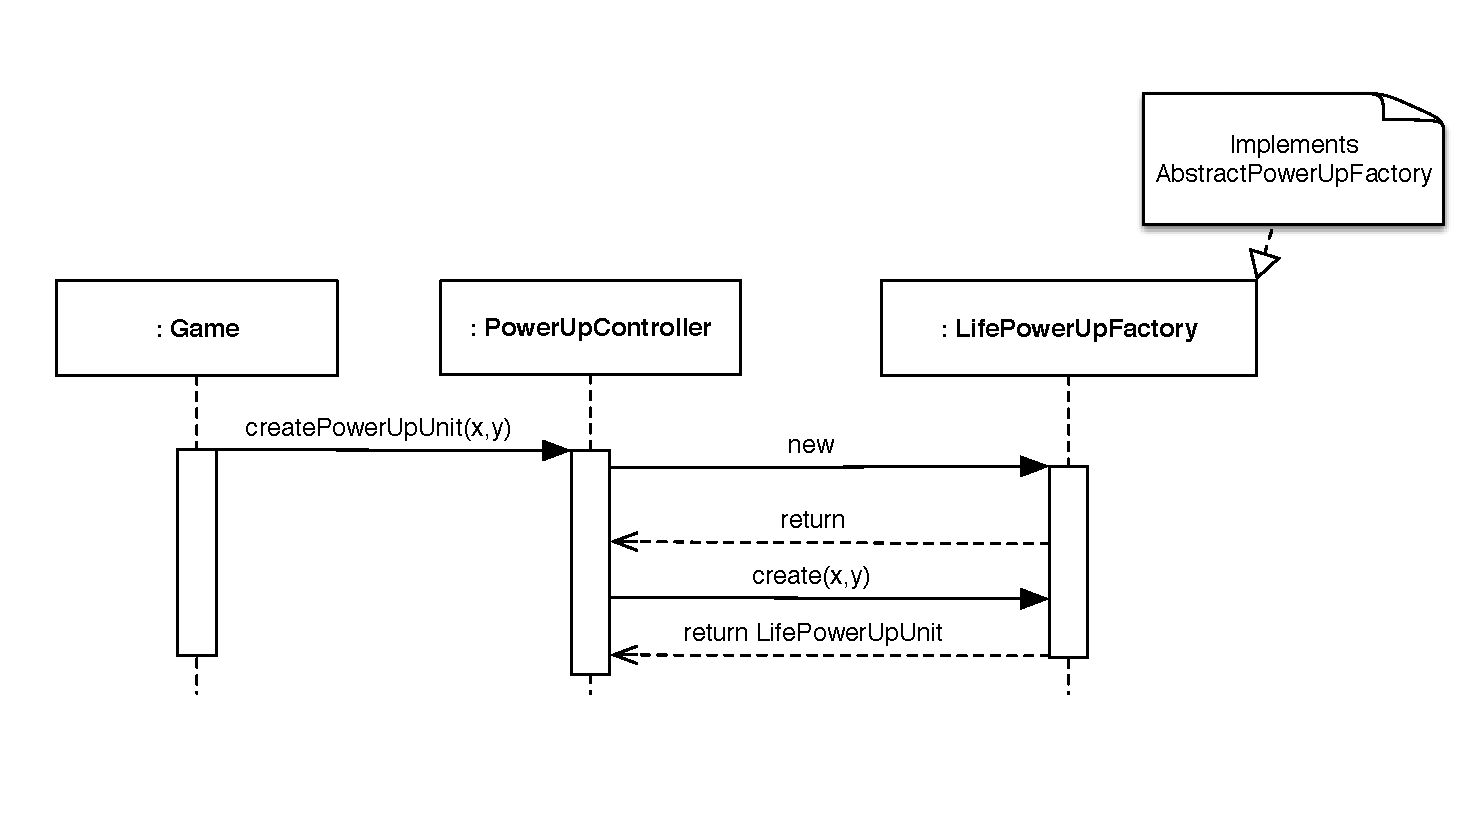
\includegraphics[width=15cm]{SI-Sequence-Factory.pdf}
\caption{Abstract Factory Pattern UML Sequence Diagram}
\label{fig:2-3factory}
\end{figure}

Figure \ref{fig:2-3factory} contains the UML Sequence diagram for the abstract factory pattern concerning the powerups. It only contains the case of a Life powerup. Since the selection of these powerups is random, each time this sequence is visited, one of three powerup factories may appear.